% !TEX TS-program = pdflatex
% !TEX encoding = UTF-8 Unicode
% !TEX ROOT = main.tex

\vspace{4cm}

\begin{center}
  C ommt gerne wieder! \\
  H ier war es so schön mit euch. \\
  R echt viel Zeit hatten wir leider nicht, aber \\
  I rgendwie hat die Uni jetzt ein anderes Gesicht für mich. \\
  S eit stolz auf euch, dass ihr das hingekriegt habt.
\begin{center}

\end{center}
  I nnerhalb der letzten Monate hatte ich mich auch mal keinen Bock, aber \\
  S olange ich wusste für wen ich das alles mache. \\
  T ut mir den Gefallen und lest den Reader wenigstens.
\begin{center}

\end{center}
  D ie nächste ZaPF wird grandios ohne Frage! \\
  E ine ZaPF in meiner Uni mit lauter Freunden \\
  R setzt sie aber nie!
\begin{center}

\end{center}
  G ut, es war echt eine Menge Arbeit. \\
  E ntscheidungen waren unverständlich, \\
  I mmer wieder die gleichen Argumente und ich frag mich: \\
  L iest das eigentlich irgendwer? \\
  S o manch eine Zugfahrt ist draufgegangen, aber es war \\
  T ausend mal die Arbeit wert. \\
  E in Hoch auf die \textbf{\textit{\#ZAPFinHD}} \\

  \textbf{!!!}

  \vspace{1cm}
  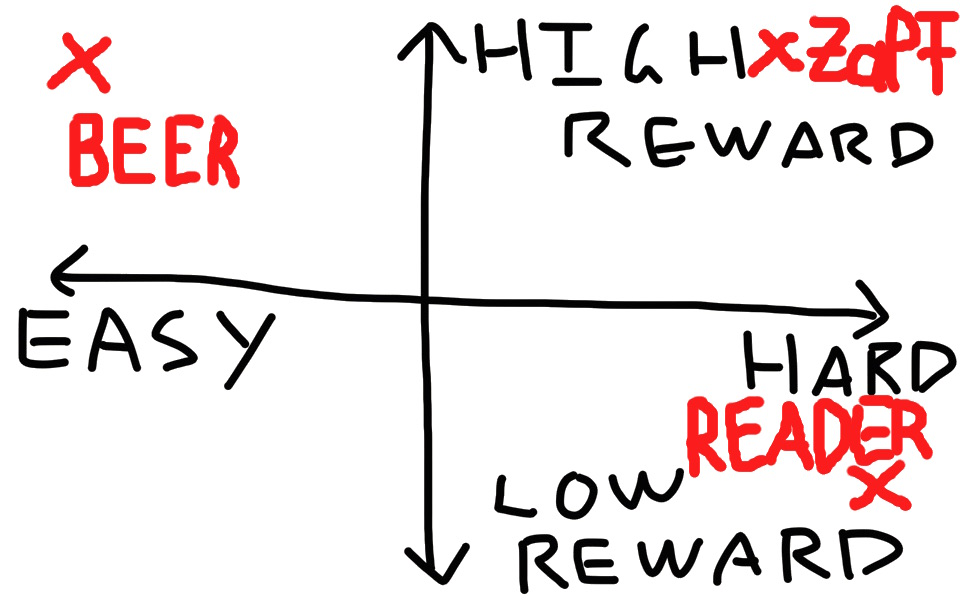
\includegraphics[scale=0.2]{bilder/readergraphic.jpg}

\end{center}

